\chapter{Literature Review} \label{LiteratureReview}
We are going to divide the classic algorithms into four sections following the model from \cite{gonzalez2016review}: \hyperref[A. Graph search planners]{Graph Search Planners} (Section \ref{A. Graph search planners}), \hyperref[B. Sampling based planners]{Sampling Based Planners} (Section \ref{B. Sampling based planners}), \hyperref[C. Interpolating curve planners]{Interpolating Curve Planners} (Section \ref{C. Interpolating curve planners}), \hyperref[D. Numerical optimization approaches]{Numerical Optimization Approaches} (Section \ref{D. Numerical optimization approaches}).
%\begin{enumerate}[label=\Alph*.]
%    \item \hyperref[A. Graph search planners]{Graph search planners}
%    \item \hyperref[B. Sampling based planners]{Sampling based planners}
%    \item \hyperref[C. Interpolating curve planners]{Interpolating curve planners}
%    \item \hyperref[D. Numerical optimization approaches]{Numerical optimization approaches}.
%\end{enumerate}

When discussing each algorithm, we are going to state how it solves the problem, how it is implemented, optimality conditions, worst case time and space complexity analysis and some of the advantages and disadvantages.

%When discussing about each algorithm we are going to describe each solution by stating how it solves the problem and state some of the advantages or disadvantages. %if it is an efficient solution (optimality, energy efficiency, computational cost). %At the end of the \hyperref[LiteratureReview]{Literature Review} section we are going to compare the performance of all algorithms.

However, before starting, let us quickly formalise the pathfinding problem so that we will have a standard notation throughout the review. We have an agent $A$ that wants to get to a goal $G$ and a set of obstacles $Os$ which the agent tries to avoid. Each of the entities belongs to a map $M=(A, Os, G)$. The purpose of the algorithm is to produce a trace, denoted by $T$, which represents the history of the agent moves from the initial agent position to the goal position. The agent can move one step at a time to a position that is valid within the map (not out of bounds or not colliding with any obstacles). The goal is reached by the agent only when the agent position matches the goal position exactly. Furthermore, we are going to assume that the environment is static and fully discovered (the algorithm does not need to explore the map while searching for a solution).

As a general rule, when we inspect the map figures, the entities will be represented by circles or squares. The colour convention will be the following: the agent is red, the initial agent position is dark red, obstacles are black, the goal is dark green (or magenta in some maps where the goal is not noticeable), the trace is light green, and the clear path is white. All map figures have been generated using the simulator from \hyperref[Simulation Platform]{PathBench} (Section \ref{Simulation Platform}).

\section{Graph Search Planners} \label{A. Graph search planners}
The discussed algorithms from this section represent a classic solution to the path finding problem. The majority of them require the world map to be represented as a graph or grid \cite{choset2005principles}.

A graph (See Figure \ref{fig:graphs}) is a data structure that is composed of nodes (vertices) and edges usually represented as $G = (V, E)$ where $V$ is a collection of nodes (vertices) and $E$ is a collection of edges. The edges can be undirected (undirected graph; bidirectional movement) or directed (directed graph; unidirectional movement). Each edge can have an associated weight (weighted graph) or not (unweighted graph), which might represent the movement cost between two nodes \cite{choset2005principles}.

\begin{figure}[h!]
  \centering
  \begin{subfigure}[b]{0.18\linewidth}
    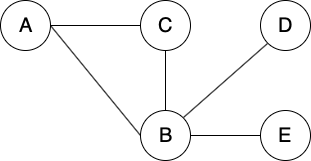
\includegraphics[width=\linewidth]{images/undirected_unweighted_graph.png}
     \caption{Undirected unweighted graph}
  \end{subfigure}
  \hfill
  \begin{subfigure}[b]{0.18\linewidth}
    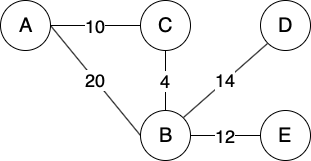
\includegraphics[width=\linewidth]{images/undirected_weighted_graph.png}
    \caption{Undirected weighted graph}
  \end{subfigure}
  \hfill
  \begin{subfigure}[b]{0.18\linewidth}
    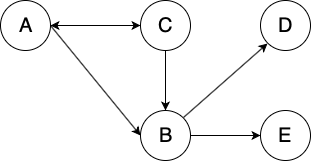
\includegraphics[width=\linewidth]{images/directed_unweighted_graph.png}
    \caption{Directed unweighted graph}
  \end{subfigure}
  \hfill
  \begin{subfigure}[b]{0.18\linewidth}
    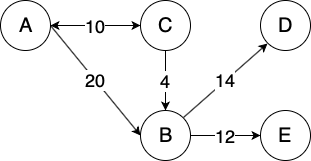
\includegraphics[width=\linewidth]{images/directed_weighted_graph.png}
    \caption{Directed weighted graph}
  \end{subfigure}
  \caption{Graph examples. The nodes are represented with a circle, and the identifier is the letter inside them. The edges are represented by lines or arrows, and the values from them represent weight values}
  \label{fig:graphs}
\end{figure}

A grid (See Figure \ref{fig:grids}) is a two-dimensional table that allows movement to nearby cells. This data structure can be easily translated to an undirected unweighted graph where grid cells represent nodes and neighbours represent undirected edges. The neighbours are defined in terms of the grid connectivity type which can be 4-point connectivity (up, down, left, right) or 8-point connectivity (all 4-point connectivity neighbours, principal diagonal and secondary diagonal) \cite{choset2005principles}. We are going to assume 8-point connectivity for all grids unless explicitly stated.

\begin{figure}[h!]
  \centering
  \begin{subfigure}[b]{0.18\linewidth}
    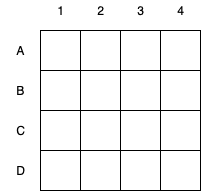
\includegraphics[width=\linewidth]{images/4x4_grid.png}
     \caption{4$\times$4 normal grid\newline\newline}
  \end{subfigure}
  \hfill
  \begin{subfigure}[b]{0.18\linewidth}
    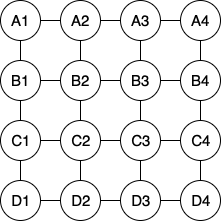
\includegraphics[width=\linewidth]{images/4_way_graph.png}
    \caption{4-point connectivity graph representation}
  \end{subfigure}
  \hfill
  \begin{subfigure}[b]{0.18\linewidth}
    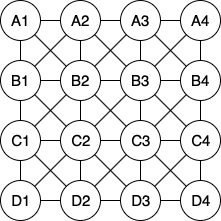
\includegraphics[width=\linewidth]{images/8_way_graph.png}
    \caption{8-point connectivity graph representation}
  \end{subfigure}
  \caption{4x4 grid example with associated 4-point and 8-point connectivity graphs. In 4-point connectivity, the neighbours are up, down, left and right. In 8-point connectivity, the neighbours are all 4-point connectivity neighbours, the principal diagonal and the secondary diagonal. The numbers at the top and left of the grid represent coordinates}
  \label{fig:grids}
\end{figure}

A tree (See Figure \ref{fig:trees}) is a directed graph with a root (i.e. a node that has no incoming edges) where each node has directed edges to their children. A particular property of the tree is that it contains no cycles. This data structure is essential as most algorithms have to walk the graph in some way (depth-first search, breadth-first search) in order to discover a possible path. Depth-first search (DFS) \cite{Cormen:2009:IAT:1614191} is a graph walking method that can be implemented using a stack (Last In First Out (LIFO) data structure) or recursion (stack is preferred, due to the recursion depth constraint that most programming languages incorporate). DFS starts by “expanding” the root (i.e. visit the node and push the node’s children onto the stack) and then iteratively expands the latest node from the stack. Thus, we initially visit the first children of the node we expand and then visit its children recursively before continuing with the second child. Breadth-first search (BFS) \cite{Cormen:2009:IAT:1614191} is another graph walking method that uses a queue (First In First Out FIFO data structure). BFS starts by expanding the root and then it repeats the process iteratively for the children. Thus we first visit \textbf{all} of the children of the node we expand and then we continue to expand each child. When BFS has to expand a node, it chooses the one in the front of the queue, and then it puts \textbf{all} of the children at the end of the queue. The result of both methods is a tree \cite{choset2005principles}.

\begin{figure}[h!]
  \centering
  \begin{subfigure}[b]{0.18\linewidth}
    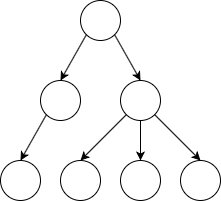
\includegraphics[width=\linewidth]{images/tree_example.png}
     \caption{A tree}
  \end{subfigure}
  \hfill
  \begin{subfigure}[b]{0.18\linewidth}
    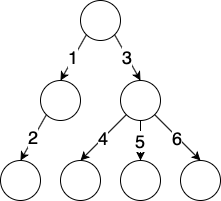
\includegraphics[width=\linewidth]{images/dfs.png}
    \caption{DFS walk}
  \end{subfigure}
  \hfill
  \begin{subfigure}[b]{0.18\linewidth}
    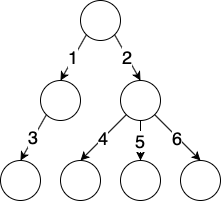
\includegraphics[width=\linewidth]{images/bfs.png}
    \caption{BFS walk}
  \end{subfigure}
  \caption{An example of a tree along with a DFS and BFS walk. The numbers indicate the order of expansions}
  \label{fig:trees}
\end{figure}

The worst case time complexity of DFS is $\mathcal{O}(b^d)$ and the worst case space complexity is $\mathcal{O}(b \cdot d)$ if a stack is used and $\mathcal{O}(d)$ if recursion is used, where $b$ is the branching factor (the average number of a node's children) and $d$ is the visiting depth. Time complexity is trivial as at each step we run a new search for all the node children $b$, and we do this $d$ times. If we use a stack, for each node, we push all children onto the stack. We do this $d$ times, and each node has $b$ children. Therefore the space complexity is $\mathcal{O}(b \cdot d)$. When using recursion, the space complexity is lower as it is defined in terms of the recursion depth (we do not use all children at once at each recursion step). However, we still prefer to use the stack in practice, due to the programming language limitations \cite{Cormen:2009:IAT:1614191}.

The worst case time and space complexity of BFS is $\mathcal{O}(b^d)$. The time complexity follows the same reasoning as DFS. Space complexity is given by the number of nodes in the queue at one time which is equal to the number of the nodes on each layer of the tree which is $\mathcal{O}(b^d)$ as each layer node count grows exponentially \cite{Cormen:2009:IAT:1614191}.

When talking about complexities we have opted for the $b$ (branching factor) and $d$ (depth) notation instead of the $|E|$ (number of edges) and $|V|$ (number of vertices/nodes) (e.g. DFS space complexity is the same as BFS space complexity $\mathcal{O}(|V|)$). We are going to discuss algorithms which attempt to prune the search space, and we can infer more information from the first notation rather than the second one \cite{Cormen:2009:IAT:1614191}.

In practice, we prefer to use BFS when dealing with problems that attempt to find an optimal solution (due to the visiting pattern) and DFS when we want to visit the whole tree without caring about the visiting pattern or when we have memory constraints.

\subsection{Wave-front Planner} \label{sec: wave-front}
The Wave-front Planner algorithm \cite{choset2005principles, luo2014effective} (See Figure \ref{fig:wave_front_planner}) is one of the simplest solutions to the pathfinding problem. The algorithm can only run on grids (two dimensional or higher). The main idea is to have a separate grid with initial values of 0 then "propagate" a wave from the goal position to the agent position. Thus, we essentially create a potential function on the grid. 

The wave is propagated by applying BFS to the separate grid from the goal position and then labelling the nodes on the same level of the tree with the level number. Thus, we first visit all the (valid) neighbours of the goal and mark the positions on the new grid with a 2 (as the goal position is marked with 1). Then we repeat the process for the nodes labelled with a 2 by expanding them and marking their \textbf{not visited} neighbours with a 3. The process is repeated until we hit the agent position. After that, we apply gradient descent from the agent position to the goal position. We start from the agent marked with number $x$ and then search its neighbours for a node marked with $x-1$. If there are multiple choices we can choose a random number as the invariant of the algorithm states that, given any node, the distance between itself and the agent is the absolute difference between their grid values (See Algorithm \ref{alg: wave_front_planner}).

% figures align
\vspace{-0.5cm}
$$dist(n) = abs(grid(G) - grid(n))$$
\vspace{-0.5cm}

We can easily prove that the algorithm finds the optimal solution in terms of minimum distance as we have used BFS to expand the nodes. If we would have used DFS instead, we could have still found a solution, but it would not necessarily be optimal due to the visiting pattern in DFS. The path might not be optimal in environments where the edge transition cost is not equal in all directions (e.g. moving on the diagonal ($\sqrt{2}$) is more expensive than moving vertically or horizontally (1) based on the Euclidean distance).

The worst case time and space complexity are given by the visiting method (BFS in our case) which is $\mathcal{O}(b^d)$, where $b$ is the branching factor, and $d$ is the depth of the solution (\textit{Get-Backtrace} is $\mathcal{O}(d)$).

One of the major drawbacks to this approach is that the optimal path is dangerously close to the obstacles (as only the attraction function is used) and in the real world, it might lead to collisions. It is also computationally expensive as the planner's search space is quite large since it does not apply any pruning. Moreover, the time and space complexity increase exponentially with the dimension of the environment. In a 2D grid with 8-point connectivity $b$ is 8, but in a 3D grid world $b$ is $3 \times 9 - 1 = 26$ (we subtract the (0, 0, 0) direction), where $b$ is the branching factor. A nice way to visualise the increase of $b$ is to count the number of combinations on each direction. Each coordinate has 3 configurations (1, 0, -1) and the number of combinations is given by $3^D$, where $D$ is the dimension. Therefore, $b = 3^D - 1$ (we have to subtract the (0, 0, ..., 0) configuration as it is not a valid neighbour). Therefore, time and space complexity becomes $\mathcal{O}((3^D)^d)$. However, because we are working with real-world robots, we can only consider 2D and 3D environments (2D for ground robot, 3D for drones and flying robots).

% A possible memory optimisation is to use the same input grid if the grid entities are labelled with a number (0 clear, 1 wall, -1 agent, 2 goal). However one requirement is that the goal has to be identified with a number higher then all other available entities.

\begin{figure}[]
  \centering
  \begin{subfigure}[b]{0.2\linewidth}
    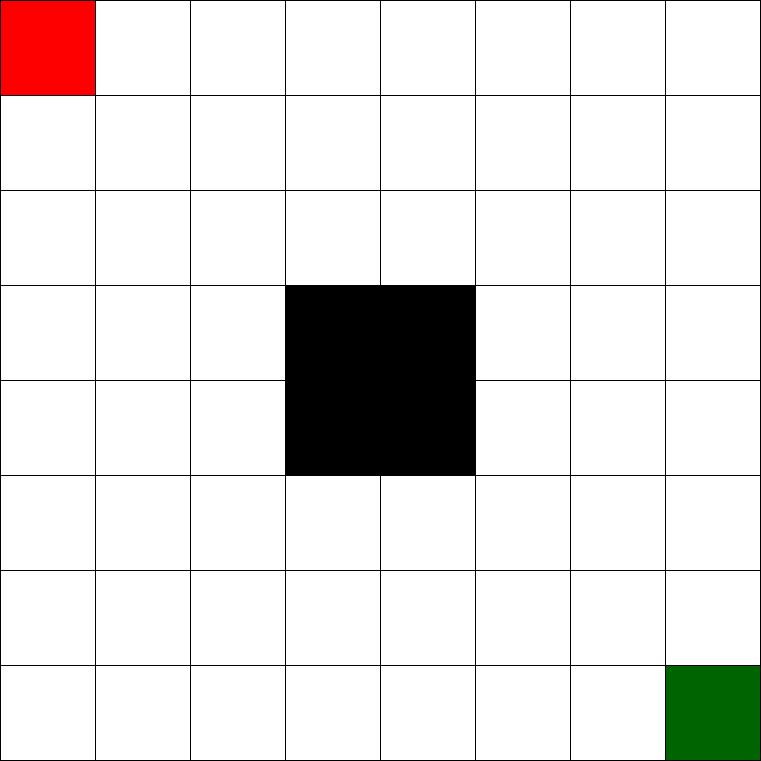
\includegraphics[width=\linewidth]{images/simple_grid.png}
     \caption{Starting 8x8 grid}
  \end{subfigure}
  \hfill
  \begin{subfigure}[b]{0.2\linewidth}
    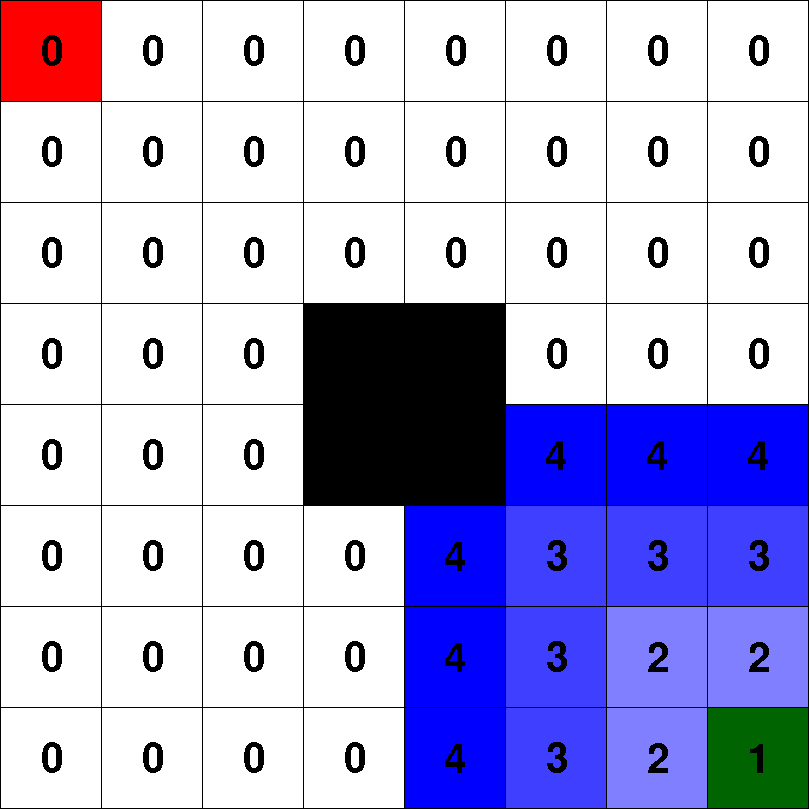
\includegraphics[width=\linewidth]{images/wave_front_planner_1.png}
     \caption{Iteration 1}
  \end{subfigure}
  \hfill
  \begin{subfigure}[b]{0.2\linewidth}
    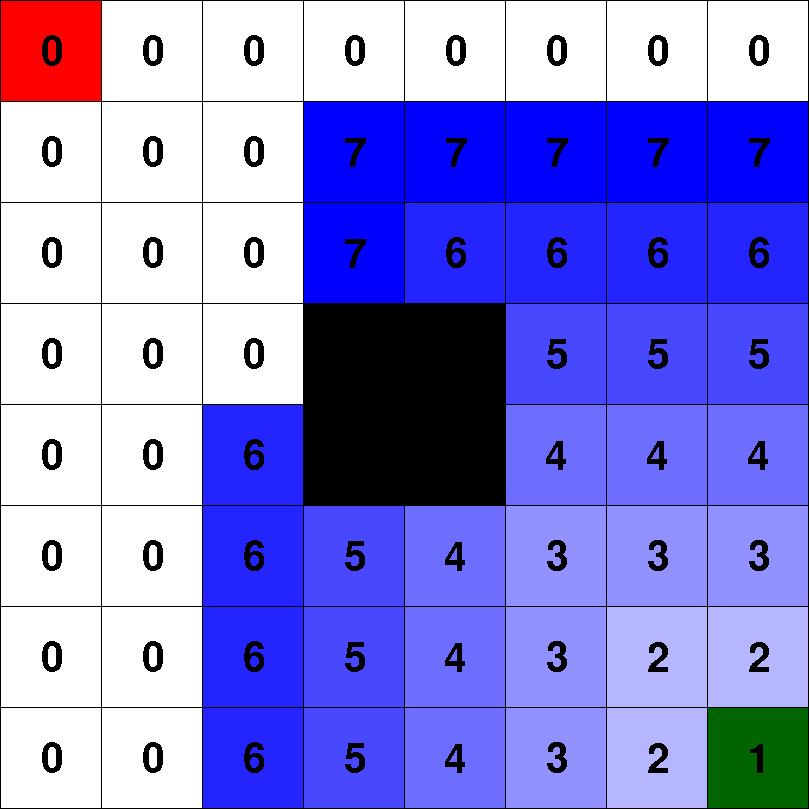
\includegraphics[width=\linewidth]{images/wave_front_planner_2.png}
    \caption{Iteration 2}
  \end{subfigure}
  \hfill
  \begin{subfigure}[b]{0.2\linewidth}
    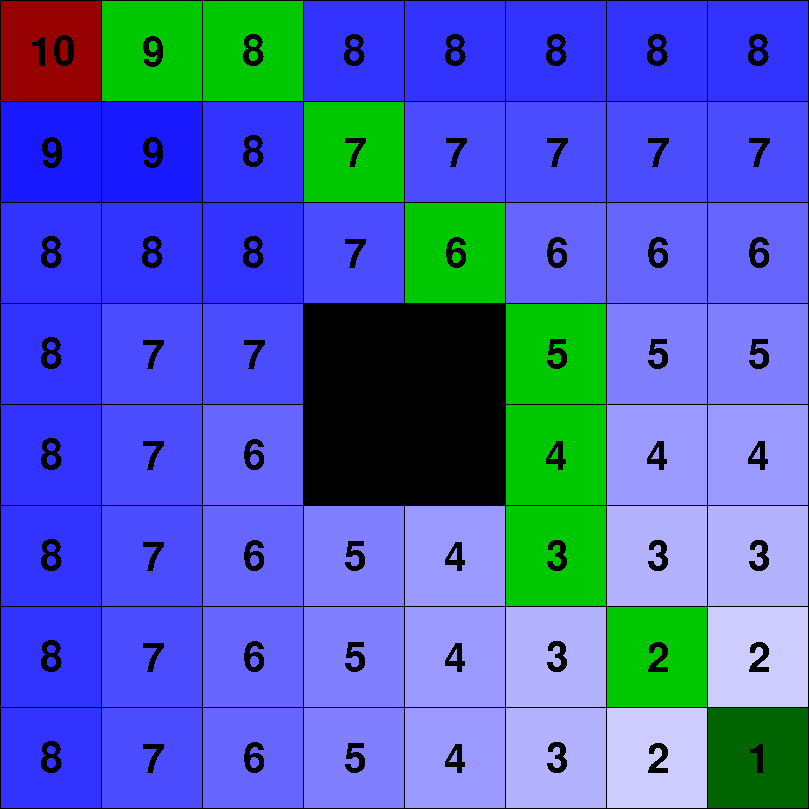
\includegraphics[width=\linewidth]{images/wave_front_planner_3.png}
    \caption{Final trace}
  \end{subfigure}
  \caption{Wave-front Planner algorithm run on an 8x8 grid (4 iteration points shown: start, 1, 2, final trace). The red square represents the agent start position, the dark green square represents the goal position, black squares represent obstacles, white squares represent the clear path, light green squares represent the final path chosen by the algorithm. The numbers in each grid cell represent the gradient map and the white (min) - dark blue (max) gradient colour is another representation of the gradient map}
  \label{fig:wave_front_planner}
\end{figure}

\begin{algorithm}[h!]
\caption{Wave-Front Planner}
\label{alg: wave_front_planner}
\begin{algorithmic}[1]

\Procedure{Get-Backtrace}{$step\_grid$, $M\colon(A, Os, G)$}
    \State $trace \gets [A]$
    % \State
    \While {$current$ is not $A$}
        \State $current \gets \forall n \in Neighbours(current). step\_grid[n] = step\_grid[current] - 1$
        \State add $current$ to $trace$
    \EndWhile
    % \State
    \State \Return $trace$
\EndProcedure
\\
    
\Procedure{Wave-Front-Planner}{$M\colon(A, Os, G)$}
    \State Initialize queue $q$ with (1, $G$)
    \State Initialize $step\_grid$ as array with same size as map
    \State $visited \gets \{\}$
    \State
    \Repeat
        \State ($current\_count$, $current\_node$) $\gets$ pop front $q$
        \State add $current\_node$ to $visited$
        \State $step\_grid[current\_node]$ $\gets$ $current\_count$
        \State
        \If {$current\_node$ is $A$}
            \State follow $\textit{Get-Backtrace}(step\_grid, M)$
            \State \Return 
        \EndIf
        \State
        \For {\textbf{each} $neighbour$ in $Neighbours(current\_node)$}
            \If {$neighbour$ is not in $visited$}
                \State append ($current\_count$ + 1, $neighbour$) to $q$
            \EndIf
        \EndFor
    \Until $q$ is empty
    \State
    \State goal was not found
\EndProcedure
\end{algorithmic}
\end{algorithm}

\subsection{A*} \label{sec:a_star}
The A* algorithm \cite{choset2005principles, duchovn2014path, zhang2014multiple, 5937169} (See figures \ref{fig:a_star}, \ref{fig:a_star_expansion}) is mostly designed to run on weighted graphs, but can be adapted to run on grids as well if we convert the grid to a graph with weights based on the Euclidean distance (1 for vertical/horizontal movement and $\sqrt{2}$ for diagonal movement).

The difference between A* and Wave-front Planner is that A* aims to prune the search space by using a heuristic function $h$ which is usually the Euclidean distance (8-point connectivity) or the Manhattan distance (4-point connectivity) (See Figure \ref{fig:distances}).

\begin{figure}[h!]
  \centering
  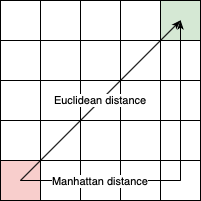
\includegraphics[scale=0.5]{images/distances.png}
  \caption{Euclidean and Manhattan distances. Red square is agent and green square is goal}
  \label{fig:distances}
\end{figure}

It is implemented using a priority queue in which the priorities are a function $f(n) = g(n) + h(n)$, where $h$ is the heuristic function mentioned above and $g$ is a function which represents the total actual distance travelled from the agent to the node $n$. The cost function $c(x, y)$ returns the graph weight cost from node $x$ to node $y$ ($x$ and $y$ have to be connected). The algorithm starts with the agent node in the priority queue. Then, the element with the highest priority (i.e. lowest $f(n)$) is picked and expanded, and its children are inserted into the priority queue. Each child will have a parent $p$, which will help us trace back the path at the end. When we expand a child we set $p(child) = n$. If a path is found, we update the goal parent. We stop the process only when the priority queue is empty or when the next priority is less than or equal to the optimal distance found. All expanded nodes are marked as seen, so we do not have to revisit them. When we expand a node, if any of its children are already in the queue we add them again if the path through the current node gives a higher priority ($g(n) < g(child)$) and update the child's parent ($p(child) = n, g(child) = g(n) + c(n, child)$). It does not matter if we add the children again to the queue as we know that $f_{cur}(child) < f_{old}(child)$ so we will visit the higher priority option first. When we stop, we compute the trace by recursively looking at the next parent from the goal until we find the agent (See Figure \ref{fig:a_star_expansion}, Algorithm \ref{alg: a_star}).

A* finds the shortest path, if and only if, the heuristic function is optimistic. An optimistic heuristic function is always less than or equal to the shortest distance.

The worst case time and space complexity of A* is $\mathcal{O}(b^d)$, where $b$ is the branching factor, and $d$ is the depth of the solution because the underlying algorithm structure is similar to BFS (\textit{Get-Backtrace} is $\mathcal{O}(d)$). However, by using a good heuristic function, the time and space complexity becomes $\mathcal{O}(\hat{b}^d)$ where $\hat{b}$ is the reduced branching factor (i.e. A* prunes the search).

% \todo{Cite wikipedia and stackoverflow??}
% https://en.wikipedia.org/wiki/A*_search_algorithm
% https://cs.stackexchange.com/questions/56176/a-graph-search-time-complexity

The significant advantage of A* is that the search space is pruned quite a lot, but it still shares the same issue as the other graph search planners: the search space grows exponentially with the grid dimension.

One of the major drawbacks is that it is not trivial to find a proper heuristic function for some environments (e.g. maps that do not define a metric space such as networks). In general, the Euclidean distance or the Manhattan distance are good choices for the heuristic function. Lastly, A* is an offline method (the internal state of the algorithm cannot be externally modified) meaning that external updates to the map are forbidden. Therefore, offline algorithms such as A* do not support dynamic and partial knowledge environments.

\pagebreak

\begin{figure}[h!]
  \centering
  \begin{subfigure}[b]{0.2\linewidth}
    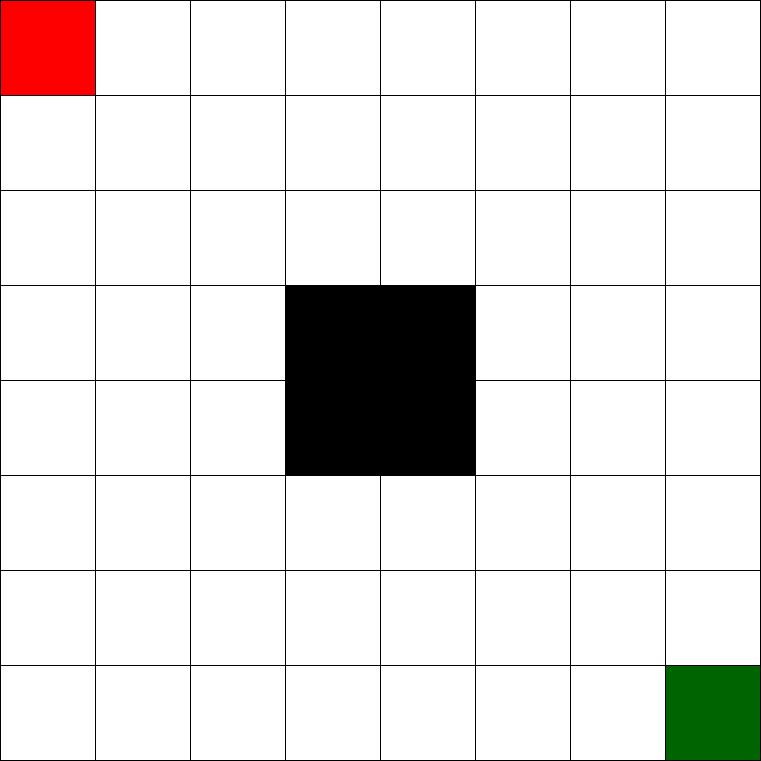
\includegraphics[width=\linewidth]{images/simple_grid.png}
     \caption{Starting 8x8 grid}
  \end{subfigure}
  \hfill
  \begin{subfigure}[b]{0.2\linewidth}
    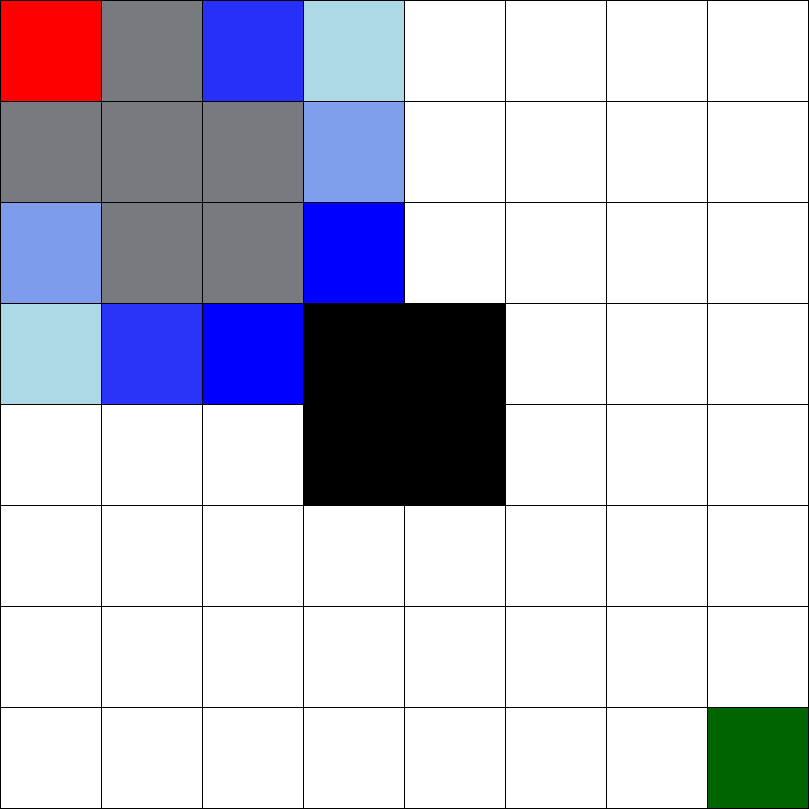
\includegraphics[width=\linewidth]{images/a_star_1.png}
     \caption{Iteration 1}
  \end{subfigure}
  \hfill
  \begin{subfigure}[b]{0.2\linewidth}
    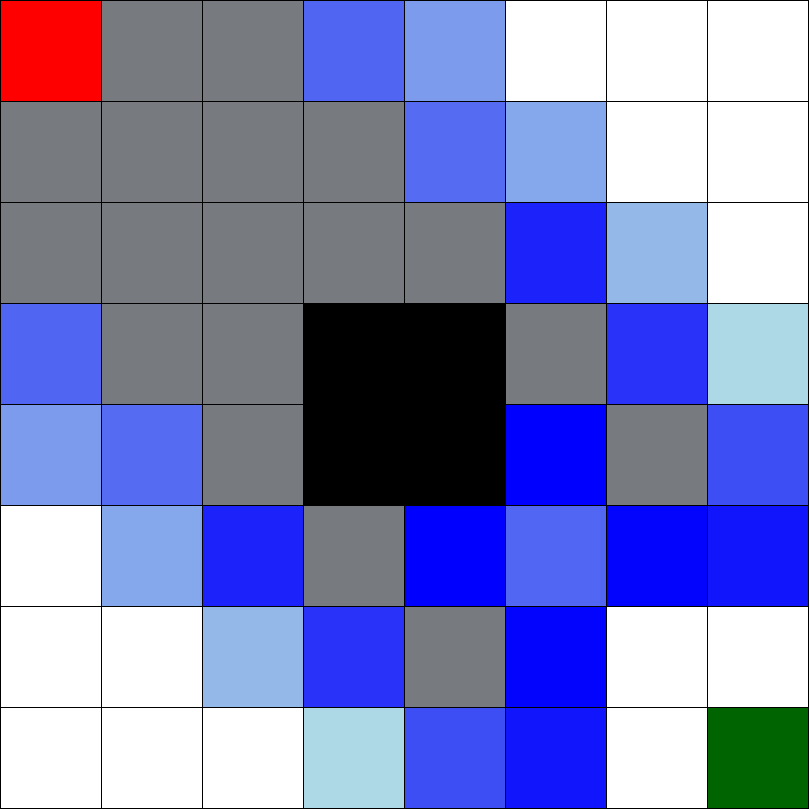
\includegraphics[width=\linewidth]{images/a_star_2.png}
    \caption{Iteration 2}
  \end{subfigure}
  \hfill
  \begin{subfigure}[b]{0.2\linewidth}
    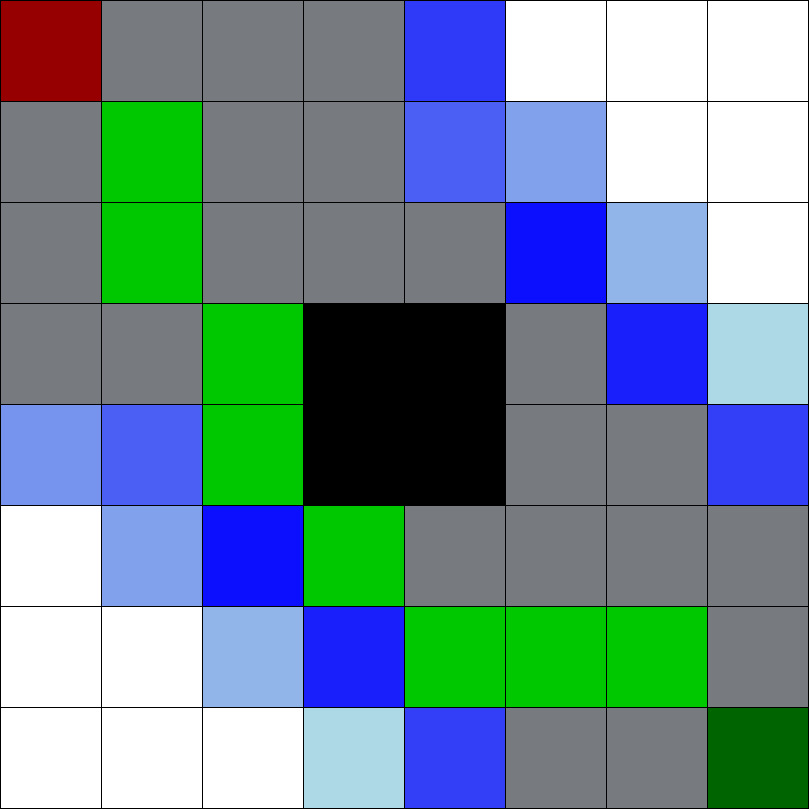
\includegraphics[width=\linewidth]{images/a_star_3.png}
    \caption{Final trace}
  \end{subfigure}
  \caption{A* algorithm run on an 8$\times$8 grid (4 iteration points shown: start, 1, 2, final trace). The red square represents agent start position, the dark green square represents the goal position, black squares represent obstacles, white squares represent the clear path, light green squares represent the final path chosen by the algorithm. The dark grey squares represent the visited set, and the blue squares represent the priority queue (the darker the blue, the higher the priority)}
  \label{fig:a_star}
\end{figure}

\begin{figure}[h!]
  \centering
  \begin{subfigure}[b]{0.2\linewidth}
    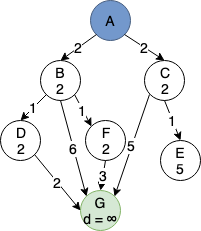
\includegraphics[width=\linewidth]{images/a_star_expansion1.png}
     \caption{Iteration 1}
  \end{subfigure}
  \hfill
  \begin{subfigure}[b]{0.2\linewidth}
    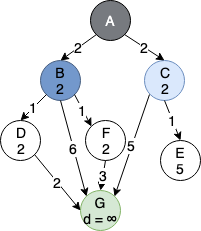
\includegraphics[width=\linewidth]{images/a_star_expansion2.png}
     \caption{Iteration 2}
  \end{subfigure}
  \hfill
  \begin{subfigure}[b]{0.2\linewidth}
    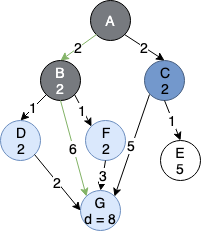
\includegraphics[width=\linewidth]{images/a_star_expansion3.png}
    \caption{Iteration 3}
  \end{subfigure}
  \newline
  \begin{subfigure}[b]{0.2\linewidth}
    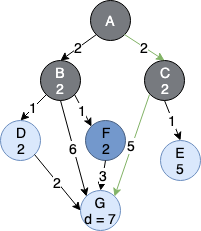
\includegraphics[width=\linewidth]{images/a_star_expansion4.png}
     \caption{Iteration 4}
  \end{subfigure}
  \hfill
  \begin{subfigure}[b]{0.2\linewidth}
    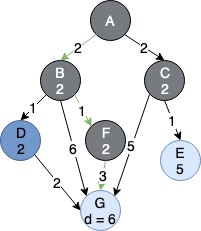
\includegraphics[width=\linewidth]{images/a_star_expansion5.png}
     \caption{Iteration 5}
  \end{subfigure}
  \hfill
  \begin{subfigure}[b]{0.2\linewidth}
    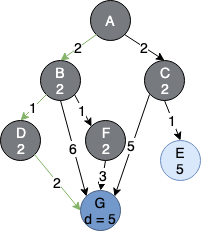
\includegraphics[width=\linewidth]{images/a_star_expansion6.png}
    \caption{Iteration 6}
  \end{subfigure}
  \hfill
  \begin{subfigure}[b]{0.2\linewidth}
    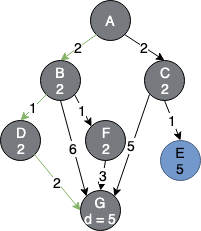
\includegraphics[width=\linewidth]{images/a_star_expansion7.png}
    \caption{Iteration 7}
  \end{subfigure}
  \caption{A* algorithm run on a directed weighted graph. Nodes are labelled with a letter that represents its name (A and G are special nodes agent and goal respectively) and the optimistic heuristic value. Edges have an associated value with them, which represents the actual distance between them. The green node is the goal, dark grey nodes are visited nodes, light blue and dark blue nodes are belonging to the priority queue, dark blue nodes are the next nodes to be expanded, green arrow trace is the optimal solution so far and $d = x$ label is optimal total distance so far}
  \label{fig:a_star_expansion}
\end{figure}

\pagebreak

\begin{algorithm}[h!]
\caption{A*}
\label{alg: a_star}
\begin{algorithmic}[1]

\Procedure{Get-Backtrace}{$p$, $M\colon(A, Os, G)$}
    \State $current \gets$ $G$
    \State $trace \gets [current]$
    \State
    \While {$current$ is not $A$}
        \State $current \gets p[$current$]$
        \State add $current$ to $trace$
    \EndWhile
    \State
    \State \Return reversed $trace$
\EndProcedure
\\

\Procedure{A*}{$M\colon(A, Os, G)$}
    \State Initialize priority queue $pq$ with ($f(A)$, $A$)
    \State $visited \gets \{\}$
    \State $p \gets \{\colon\}$
    \Repeat
        \State $current\_node$ $\gets$ best $n_{best}$ from $pq$ where $\forall n.f(n_{best}) \leq f(n)$
        \State add $current\_node$ to $visited$
        \State
        \If {$current\_node$ is $G$}
            \State follow $\textit{Get-Backtrace}(p, M)$
            \State \Return
        \EndIf
        \State
        \For {\textbf{each} $neighbour$ in $Neighbours(current\_node)$}
            \If {$neighbour$ is not in $visited$ \textbf{or} $g(current\_node) + c(current\_node, neighbour) < g(neighbour)$}
                \State $g(neighbour) \gets g(current\_node) + c(current\_node, neighbour)$
                \State add $neighbour$ to $pq$
                \State update $p[neighbour]$ to $current\_node$
            \EndIf
        \EndFor
    \Until $visited$ is empty
    \State
    \State goal was not found
\EndProcedure
\end{algorithmic}
\end{algorithm}

\subsection{Dijkstra} \label{sec: dijkstra}
The Dijkstra algorithm \cite{choset2005principles, zhang2014multiple} (See Figures \ref{fig:dijkstra}, \ref{fig:dijkstra_expansion}) is a variation of the A* algorithm where we omit the heuristic function ($f(n) = g(n)$). Therefore the algorithm becomes greedy, meaning that we expand the node with lowest distance from the agent position. (See Figure \ref{fig:dijkstra_expansion}). The algorithm is identical to A* (See Algorithm \ref{alg: a_star}), but with $f(n) = g(n)$. Thus, the space and time complexity is the same as A* $(\mathcal{O}(\hat{b}^d))$, but $\hat{b}$ is usually not as efficient as A*.

The major difference between A* and Dijkstra is that, because it is a greedy algorithm, once we expand the goal node, we find the final solution. The solution is optimal in terms of minimal distance because after we expand a node, its distance will not be modified in the future (the invariant holds for all nodes, not only for the goal). 

The drawback of using this method against A* is that it usually explores more than A* and thus the memory gets quite high.

\pagebreak

\begin{figure}[h!]
  \centering
  \begin{subfigure}[b]{0.2\linewidth}
    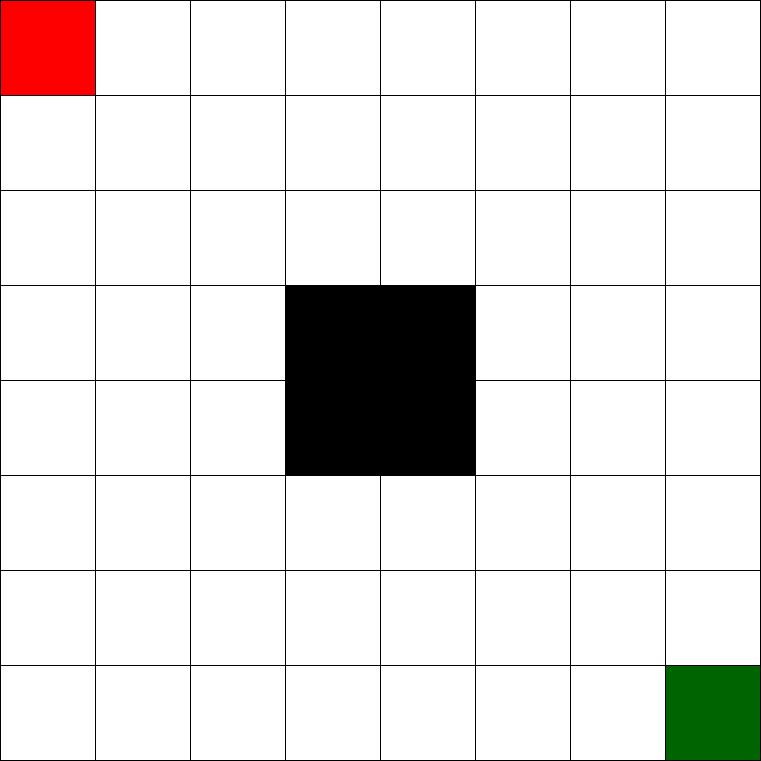
\includegraphics[width=\linewidth]{images/simple_grid.png}
     \caption{Starting 8x8 grid}
  \end{subfigure}
  \hfill
  \begin{subfigure}[b]{0.2\linewidth}
    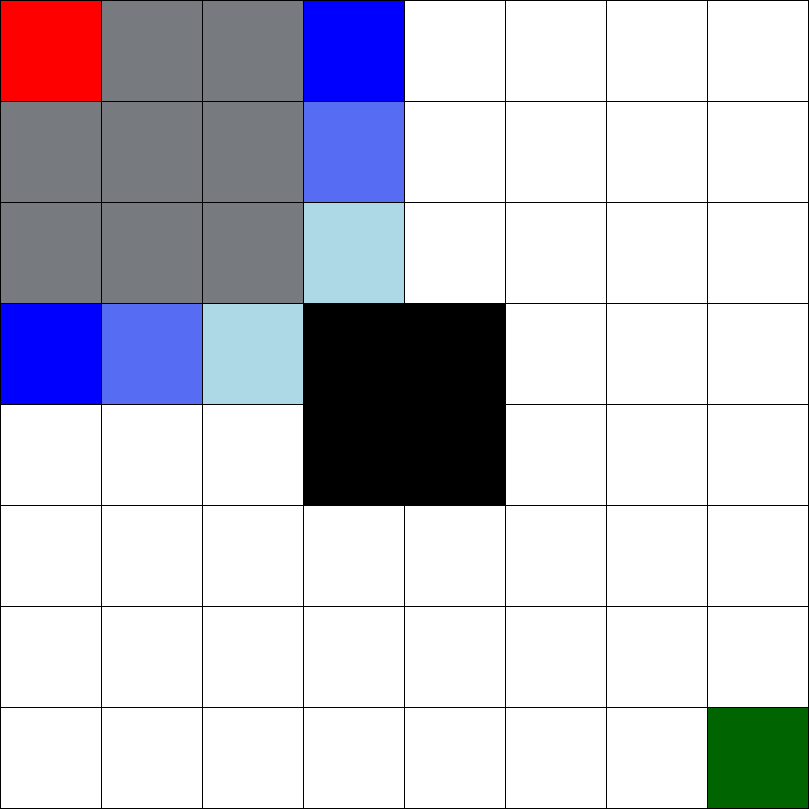
\includegraphics[width=\linewidth]{images/dijkstra1.png}
     \caption{Iteration 1}
  \end{subfigure}
  \hfill
  \begin{subfigure}[b]{0.2\linewidth}
    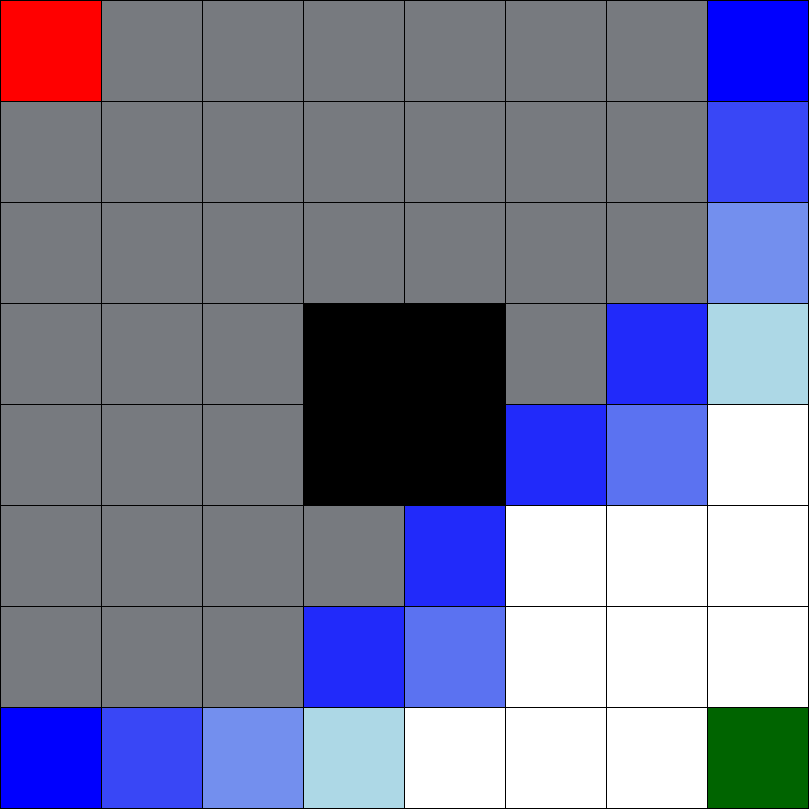
\includegraphics[width=\linewidth]{images/dijkstra2.png}
    \caption{Iteration 2}
  \end{subfigure}
  \hfill
  \begin{subfigure}[b]{0.2\linewidth}
    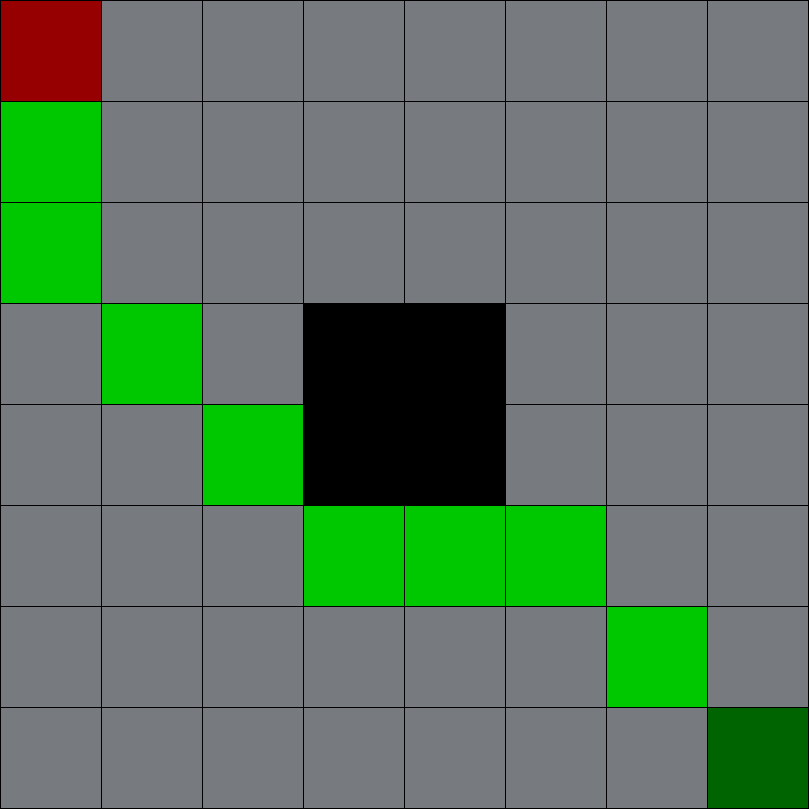
\includegraphics[width=\linewidth]{images/dijkstra3.png}
    \caption{Final trace}
  \end{subfigure}
  \caption{Dijkstra algorithm run on an 8$\times$8 grid (4 iteration points shown: start, 1, 2, final trace). The red square represents the agent start position, the dark green square represents the goal position, black squares represent obstacles, white squares represent the clear path, light green squares represent the final path chosen by the algorithm. The dark grey squares represent the visited set, and the blue squares represent the priority queue (the darker the blue, the higher the priority)}
  \label{fig:dijkstra}
\end{figure}

\begin{figure}[h!]
  \centering
  \begin{subfigure}[b]{0.2\linewidth}
    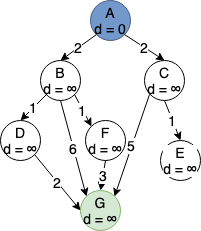
\includegraphics[width=\linewidth]{images/dijkstra_expansion1.png}
     \caption{Iteration 1}
  \end{subfigure}
  \hfill
  \begin{subfigure}[b]{0.2\linewidth}
    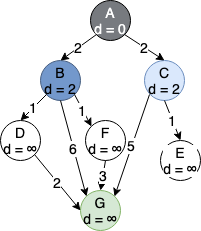
\includegraphics[width=\linewidth]{images/dijkstra_expansion2.png}
     \caption{Iteration 2}
  \end{subfigure}
  \hfill
  \begin{subfigure}[b]{0.2\linewidth}
    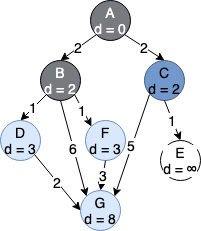
\includegraphics[width=\linewidth]{images/dijkstra_expansion3.png}
    \caption{Iteration 3}
  \end{subfigure}
  \hfill
  \begin{subfigure}[b]{0.2\linewidth}
    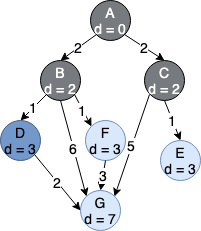
\includegraphics[width=\linewidth]{images/dijkstra_expansion4.png}
     \caption{Iteration 4}
  \end{subfigure}
  \newline
  \begin{subfigure}[b]{0.2\linewidth}
    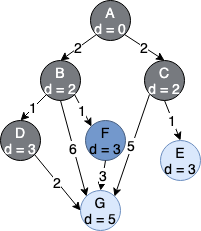
\includegraphics[width=\linewidth]{images/dijkstra_expansion5.png}
     \caption{Iteration 5}
  \end{subfigure}
  \hfill
  \begin{subfigure}[b]{0.2\linewidth}
    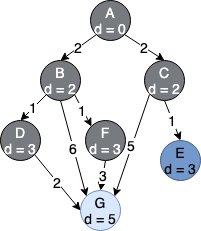
\includegraphics[width=\linewidth]{images/dijkstra_expansion6.png}
    \caption{Iteration 6}
  \end{subfigure}
  \hfill
  \begin{subfigure}[b]{0.2\linewidth}
    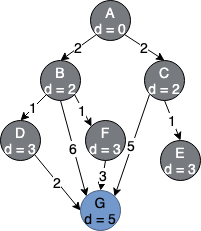
\includegraphics[width=\linewidth]{images/dijkstra_expansion7.png}
     \caption{Iteration 7}
  \end{subfigure}
  \hfill
  \begin{subfigure}[b]{0.2\linewidth}
    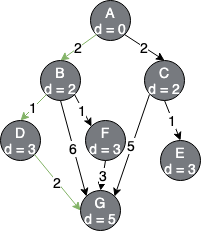
\includegraphics[width=\linewidth]{images/dijkstra_expansion8.png}
    \caption{Iteration 8}
  \end{subfigure}
  \hfill
  \caption{Dijkstra algorithm run on a directed weighted graph. Nodes are labelled with a letter identifier (A and G are special nodes agent and goal respectively) and the current distance. The distance is final when the node is marked as visited. Edges have an associated value with them, which represents edge weight. The green node is the goal, dark grey nodes are visited nodes, light blue and dark blue nodes are belonging to the priority queue, dark blue nodes are the next nodes to be expanded, green arrow trace is the optimal solution}
  \label{fig:dijkstra_expansion}
\end{figure}

\pagebreak

\subsection{Bug Algorithms}
The bug algorithms \cite{choset2005principles, rajko2001pursuit} are one of the earliest and simplest sensor-based solutions for the pathfinding problem, and we will cover two implementations: Bug1 and Bug2. There exist other algorithms which are more advanced such as Tangent Bug described in \cite{choset2005principles, rajko2001pursuit, kamon1998tangentbug}, but we will not cover them as it exceeds the scope of our report.

The idea behind bug algorithms is based on the instinctual behaviour of a bug moving directly towards a destination (goal) and turning around encountered obstacles. The algorithms have two phases: straight line movement (phase 1) and object boundary following (phase 2). We will assume that the agent has a contact sensor that detects if the agent is in the proximity of the boundary of an obstacle.

%We will cover the boundary following algorithm at the end of this section.

The bug algorithms are trivial to implement, not computationally expensive, and it has been shown that their success is guaranteed, meaning that they can find a path to the goal if one exists. However, they do not find the optimal path.

\subsubsection{Bug1} \label{sec: bug1}

First, we label the direction from the agent position to the goal position with $dir_{AG} = \frac{d(A, G)
}{\norm{d(A, G)}} = \frac{(G - A)} {\norm{G - A}}$. In the first phase, the algorithm follows $dir_{A, G}$ until an obstacle is detected and we mark this position as $P_{i}$. Afterwards, it proceeds with the second phase by doing a complete loop around the obstacle while registering the closest distance on the boundary to the goal (find $\hat{Ob} = \argmin{Ob}{d_{Ob, G}}, Ob \in Boundary(O)$) until we reach $P_{i}$. After that, we follow the boundary again until we reach $\hat{Ob}$ and return to the first phase. We repeat this process until the goal is found. If the agent were to move, but it can't from $\hat{Ob}$, then we conclude the algorithm as the goal is unreachable (See Figure \ref{fig:Bug1}, See Algorithm \ref{alg: bug1}) \cite{lumelsky1986dynamic}.

As it is quite hard to estimate the worst case time complexity, we are going to express it as the number of steps upper bound ($\mathcal{O}(upper_{Bug1})$). The upper bound on the number of steps is given by the total distance from the agent to the goal $d(A, G)$, in the case of no obstacles, plus the worst case traversed boundary length for all obstacles $1.5 \sum_{o \in O} length(Boundary(o))$. The space complexity is $\mathcal{O}(1)$ (not counting recursion steps as it can be collapsed in a while loop).

$$upper_{Bug1} = d(A, G) + 1.5 \sum_{o \in O} length(Boundary(o))$$

\begin{figure}[h!]
  \centering
  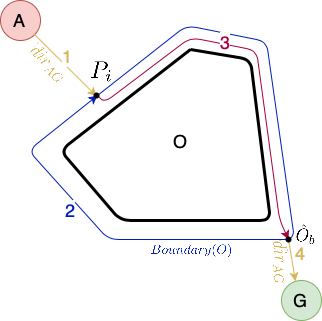
\includegraphics[scale=0.4]{images/Bug1.png}
  \caption{Bug1: Arrows represent the movement direction and numbers represent the traversal order. Yellow arrows represent the first phase. Blue and red arrows represent the second phase}
  \label{fig:Bug1}
\end{figure}

\begin{algorithm}
\caption{Bug1}
\label{alg: bug1}
\begin{algorithmic}[1]
\Procedure{Bug1}{$M\colon(A, Os, G)$}
    \State $\textit{Phase1}(M)$
\EndProcedure
\\
\Procedure{Phase1}{$M\colon(A, Os, G)$}
    \State move agent towards goal along $dir_{A, G}$ until hits $P_i$ or $G$
    \If {$G$ was reached}
        \State \Return
    \EndIf
    \State $\textit{Phase2}(M, P_i)$
\EndProcedure
\\
\Procedure{Phase2}{$M\colon(A, Os, G)$, $P_i$}
    \State find obstacle $O$ with hit point $P_i$ from $Os$
    \State do a full loop around $Boundary(O)$ while computing $\hat{O}b$
    \State follow $Boundary(O)$ until $\hat{O}b$ is reached
    \State
    \If {can't move from $\hat{Ob}$ to $G$}
        \State goal can't be reached
        \State \Return
    \EndIf
    \State
    \State $\textit{Phase1}(M)$
\EndProcedure
\end{algorithmic}
\end{algorithm}

\subsubsection{Bug2} \label{sec: bug2}
The first stage is identical to the one in Bug1, but the second stage follows a greedy approach. Instead of making a full obstacle loop in the second stage, we try to find the point $P \in Boundary(O)$ which belongs to the line segment determined by the original starting agent position and the goal position $P \in LS_{A_{initial}, G}$. $P$ should also be chosen in such a way that it is closer than the original point of contact with the obstacle $P_i$. If $P = P_i$ then the goal can't be reached (See Figure \ref{fig:Bug2}, See Algorithm \ref{alg: bug2}) \cite{lumelsky1986dynamic}.

However, this does not imply that Bug2 outperforms Bug1 in all cases. The time complexity (given as the upper bound) for Bug2 is determined by the total distance from the agent to the goal $d(A, G)$, in the case of no obstacles, plus the worst case traversed boundary length for all obstacles $0.5 \sum_{o \in O} n_{o} \cdot length(Boundary(o))$. The issue here is that, because we follow a greedy approach, we might reencounter the same obstacle, thus $n_{o}$ represents how many times we have encountered obstacle $o$. Therefore, Bug1 might yield better performance in cases where the environment contains complex obstacles. The space complexity is still $\mathcal{O}(1)$.

$$upper_{Bug2} = d(A, G) + 0.5 \sum_{o \in O} n_{o} \cdot length(Boundary(o))$$

\begin{figure}[h!]
  \centering
  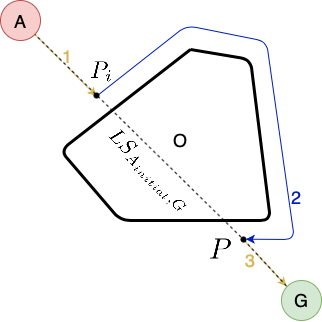
\includegraphics[scale=0.4]{images/Bug2.png}
  
  \caption{Bug2: Arrows represent the movement direction and numbers represent the traversal order. Yellow arrows represent the first phase. Blue arrows represent the second phase}
  \label{fig:Bug2}
\end{figure}

\begin{algorithm}[h]
\caption{Bug2}
\label{alg: bug2}
\begin{algorithmic}[1]
\Procedure{Bug2}{$M\colon(A, Os, G)$}
    \State $\textit{Phase1}()$
\EndProcedure
\\
\Procedure{Phase1}{$M\colon(A, Os, G)$}
    \State move agent towards goal along $LS_{A_{initial}, G}$ until hits $P_i$ or $G$
    \If {$G$ was reached}
        \State \Return
    \EndIf
    \State $\textit{Phase2}(M, P_i)$
\EndProcedure
\\
\Procedure{Phase2}{$M\colon(A, Os, G)$, $P_i$}
    \State find obstacle $O$ with hit point $P_i$ from $Os$
    \State follow $Boundary(O)$ until we hit $P \in LS_{A_{initial}, G}$, $d(P_{i}, G) \geq d(P, G)$
    \State
    \If {$P$ = $P_i$}
        \State goal can't be reached
        \State \Return
    \EndIf
    \State
    \State $\textit{Phase1}(M)$
\EndProcedure
\end{algorithmic}
\end{algorithm}

%\textbf{Tangent Bug}

%\textbf{Curve Tracing}

\subsection{Value Iteration on Markovian Decision Processes (MDP)} \label{sec:vin}
The Markovian Decision Process (MDP) \cite{szepesvari2010algorithms, satia1973markovian} (See Figure \ref{fig:MDPWorld}) represents a state environment in which an agent can transition from one state to the next one until it reaches a terminating state. Whenever the agent chooses an action by moving from a state to another, it is rewarded based on the type of action that it took and the previous and next states. 

Formally, a Markovian Decision Process is a tuple $\langle\mathcal{S}, \mathcal{A}, \mathcal{P}_{s, s'}^a, \mathcal{R}_{s, s'}^a, \gamma \in [0, 1], \pi \rangle$. $\mathcal{S}$ is the state space, $\mathcal{A}$ is the action space (what actions are available to the agent), $\mathcal{P}_{s, s'}^a$ is the probability transition matrix which gives the probability of transitioning with action $a$ from state $s$ to state $s'$, $\mathcal{R}_{s, s'}^a$ is the reward matrix and states the reward for taking action $a$ from state $s$ to state $s'$, $\gamma$ is the discounted rewards factor and $\pi$ is the policy which can be deterministic or stochastic.

\begin{figure}[h!]
  \centering
  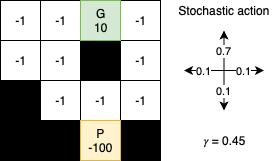
\includegraphics[scale=0.5]{images/MDPWorld.png}
  \caption{An example of an MDP world. White squares represent possible states. The agent can start from \textbf{any} of the white squares. There are 2 special terminal states: the green square represents the goal, and the yellow square represents the penalty state. Each state has an associated reward value which is collected whenever the agent leaves the state (for the terminal states, the reward is collected instantaneously). There are 4 possible actions (up, right, down, left; 4-point connectivity), but each action is stochastic meaning that if the agent chooses a specific direction it will move in that direction with 0.7 probability or it will move to the other directions with equal probability}
  \label{fig:MDPWorld}
\end{figure}

$R_t$ represents the total discounted reward from time step $t$, and it is defined in terms of the collected rewards $r_t$.

$$R_t = r_{t+1} + \gamma r_{t + 2} + \gamma^2 r_{t + 3} + ... = \sum_{k = 0}^{\infty} \gamma^k r_{t + k + 1}$$

The value function $V^{\pi}(s)$, where $\pi$ is the policy,  with signature $V^{\pi} \colon \mathcal{S} \xrightarrow{} \mathbb{R}$ represents a method for assessing how "good" a state is. It is defined as the expected total discounted reward.

$$V^{\pi}(s) = \mathbb{E}_{\pi}[R_t|S_t = s] = \sum_{a \in \mathcal{A}} \pi(s, a) \sum_{s' \in S} \mathcal{P}_{s, s'}^a (\mathcal{R}_{s, s'}^a + \gamma V^{\pi}(s'))$$

The state-action value function $Q^{\pi}(s, a)$ with signature $Q^{\pi} \colon \{ \mathcal{S}, \mathcal{A} \} \xrightarrow{} \mathbb{R}$ represents a method for assessing how "good" a state is, given a certain action.

$$Q^{\pi}(s, a) = \mathbb{E}_{\pi}[R_t|S_t = s, A_t = a] = \sum_{s' \in S} \mathcal{P}_{s, s'}^a (\mathcal{R}_{s, s'}^a + \gamma V^{\pi}(s'))$$

This also means that we can define $V^{\pi}(s)$ in terms of $Q^{\pi}(s, a)$.

$$V^{\pi}(s) = \sum_{a \in \mathcal{A}} \pi(s, a) Q^{\pi}(s, a)$$

\begin{Theo}{Bellman Optimality Equation}{Bellman}
The Bellman Optimality Equation states that the optimal value function is given by the following formula:
\begin{align*}
    V^{\pi^{*}}(s) &= \max_{a} \sum_{s' \in S} \mathcal{P}_{s, s'}^a (\mathcal{R}_{s, s'}^a + \gamma V^{\pi^{*}}(s')) = \max_{a} Q^{\pi^{*}}(s, a)\\
    Q^{\pi^{*}}(s, a) &= \sum_{s' \in S} \mathcal{P}_{s, s'}^a (\mathcal{R}_{s, s'}^a + \gamma V^{\pi^{*}}(s'))
\end{align*}
\end{Theo}

By following the Bellman Optimality Equation (\Cref{Th:Bellman}), we can devise a dynamic programming algorithm called Value Iteration. The algorithm updates $\mathcal{V^{\pi}}$ in place by applying the Bellman Optimality Equation for each state, thus finding better $\mathcal{V^{\pi}}$ on each run. We repeat the process until we see no further changes in $\mathcal{V^{\pi}}$. This means that $\mathcal{V^{\pi}}$ has converged for all $s \in \mathcal{S}$. After that, we return the optimal policy by choosing the optimal action at each state $s \in \mathcal{S}$ (See Algorithm \ref{alg: value_iteration}). If we run the algorithm on the MDP world defined in Figure \ref{fig:MDPWorld}, we will get the results presented in Figure \ref{fig:MDPResults}.

\begin{figure}[h!]
  \centering
  \begin{subfigure}[b]{0.3\linewidth}
    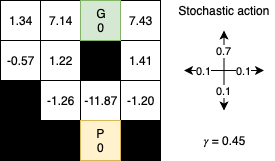
\includegraphics[width=\linewidth]{images/MDPWorldResult.png}
     \caption{Optimal value function}
  \end{subfigure}
  \hspace{1.3cm}
  \begin{subfigure}[b]{0.3\linewidth}
    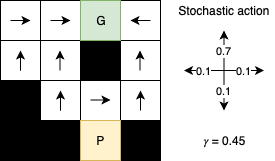
\includegraphics[width=\linewidth]{images/MDPWorldResultPolicy.png}
     \caption{Optimal policy}
  \end{subfigure}
  \caption{The results after applying the Value Iteration algorithm on the MDP World defined in figure \ref{fig:MDPWorld}. On the left, each cell contains the optimal value function $V^{\pi}(s)$. The optimal policy is displayed on the right}
  \label{fig:MDPResults}
\end{figure}

\begin{algorithm}
\caption{Value Iteration}
\label{alg: value_iteration}
\begin{algorithmic}[1]
\Procedure{Value-Iteration}{$\mathcal{S}$, $\mathcal{A}$, $\mathcal{P}$, $\mathcal{R}, \gamma$}
    \State Initialize $\mathcal{V^{\pi}}$, $\pi$ arbitrarily (e.g. all 0)
    \State
    \Repeat
        \For {\textbf{each} $s \in \mathcal{S}$}
            \State $V^{\pi}(s) = \underset{a \in \mathcal{A}}{\max} \hspace{0.1cm} \sum_{s' \in S} \mathcal{P}_{s, s'}^a (\mathcal{R}_{s, s'}^a + \gamma V^{\pi}(s'))$
        \EndFor
    \Until we have no change in $\mathcal{V^{\pi}}$
    \State
    
    \For {\textbf{each} $s \in \mathcal{S}$}
        \State $\pi(s) = \argmax{a \in \mathcal{A}}{\sum_{s' \in S} \mathcal{P}_{s, s'}^a (\mathcal{R}_{s, s'}^a + \gamma V^{\pi}(s'))}$
    \EndFor
    \State \textbf{return} $\pi$
\EndProcedure
\end{algorithmic}
\end{algorithm}

The time complexity is $\mathcal{O}(c|S||\mathcal{A}|)$ and the space complexity is $\mathcal{O}(|S|)$, where $c$ is the convergence rate, $|S|$ is the number of states and $|\mathcal{A}|$ is the number of actions. The time complexity is given by the update rule (which is $\mathcal{O}(|S||\mathcal{A}|)$, for each state we find the maximising action) being run $c$ times (some notebooks state that $c$ is bounded by $|S|$) and the final policy evaluation (which is still $\mathcal{O}(|S||\mathcal{A}|)$). The space complexity is given by the number of elements in $\mathcal{V^{\pi}}$ and $\pi$, which is the number of states $|S|$.

The advantage of using MDPs is that we can model a more complex world for the agent in which we can define areas which should be avoided (such as bridges, because they draw more battery power) by associating a negative reward with them. However, it can also be considered a disadvantage for worlds that cannot be easily modelled, as we have to know the transition probabilities and rewards apriori before we can apply Value Iteration. Not to mention that the number of states can get quite big. For instance, let us assume that we have a robotic arm with 3 joints, and each join can rotate 180\degree. If we discretise each angle into 1\degree angles, we will have a total number of $180^3 \simeq 5.8$ million states. There exist algorithms which can handle a large number of states such as Monte Carlo (sampling episode traces) and Temporal Difference Learning (combines dynamic programming and sampling), but we will not cover them as they are out of the report's scope \cite{szepesvari2010algorithms}.

\section{Sampling Based Planners} \label{B. Sampling based planners}
A significant drawback of using resolution complete (the algorithm is guaranteed to find a path) and resolution optimal (the algorithm will find the shortest path if one is available) graph search planners such as A*, is that they are only suitable for small problem sizes \cite{gammell2014informed}.

The algorithms described in this chapter employ a sampling technique to explore the unknown environment rapidly, thus scaling well with large problem sizes.

\subsection{Rapidly-exploring Random Tree (RRT)} \label{sec: RRT}
The Rapidly-exploring Random Tree (RRT) \cite{lavalle1998rapidly, rodriguez2006obstacle, lavalle2001randomized, karaman2011sampling} is a randomised data structure solution to the pathfinding problem which shares some desirable properties with probabilistic road-maps (PRM) \cite{choset2005principles}, but, unlike PRMs, it is able to handle problems that have non-holonomic constraints (a holonomic robot is a robot which is able to move instantaneously in all available degrees of freedom).

The algorithm starts by creating a graph $G$ with a single vertex containing the agent position. Then, we proceed to incrementally add new vertices until we get to the goal region (the region in which we can assume that we have reached the goal or will be able to safely reach it). At each iteration, we sample a new point on the map which represents a valid position (not intersecting any obstacle, or out of bounds) $x_{rand} \notin Os$. We find the nearest vertex $x_{near}$ from $x_{rand}$ by searching the graph (e.g. graph pruning). We choose the next vertex to be inserted $x_{new}$ based on a predefined $max\_dist$ variable. If we are too far from $x_{near}$ ($d(x_{near}, x_{rand}) > max\_dist$) we choose a point on the line segment defined by $x_{near}$ and $x_{rand}$ that is $max\_dist$ far away from $x_{near}$. If we are too close to $x_{near}$ ($d(x_{near}, x_{rand}) \leq max\_dist$) we simply choose $x_{rand}$ (See Figure \ref{fig:RRT_new_node}). After we have chosen $x_{new}$, we make sure that the path from $x_{near}$ to $x_{new}$ is collision free, and if it is we add $x_{new}$ as a new vertex to the graph $G$ and $(x_{near}, x_{new})$ as a new edge (See Figure \ref{fig:RRT_example}, See Algorithm \ref{alg: RRT}).

It is worth mentioning that there exist some variations which use a dynamic $max\_dist$, usually picking a random number from the interval $[0, max)$ at each new iteration. Furthermore, the algorithm can be extended to different metric spaces by changing the distance function $d$.

\begin{figure}[]
  \centering
  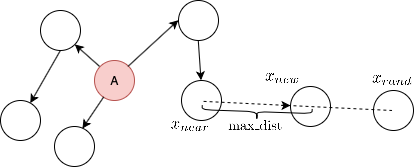
\includegraphics[scale=0.4]{images/RRT_new_node.png}
  \caption{RRT $x_{new}$ decision algorithm, if $x_{rand}$ is too far from $x_{near}$ we interpolate $x_{new}$ between the line segment defined by $x_{near}$ and $x_{rand}$ such that $x_{new}$ is $max\_dist$ away from $x_{near}$}
  \label{fig:RRT_new_node}
\end{figure}

\begin{figure}[]
  \centering
  \begin{subfigure}[b]{0.3\linewidth}
    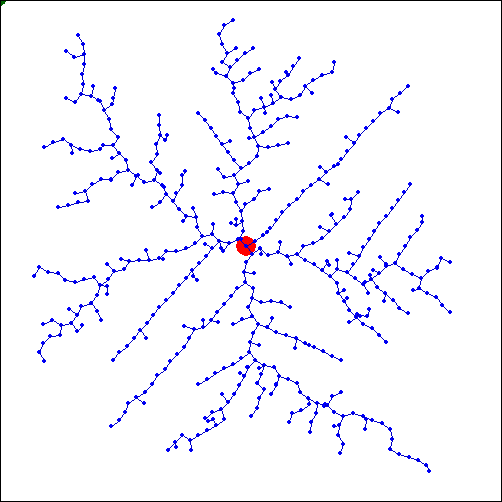
\includegraphics[width=\linewidth]{images/screenshot_40.png}
     \caption{500 iterations}
  \end{subfigure}
  \hfill
  \begin{subfigure}[b]{0.3\linewidth}
    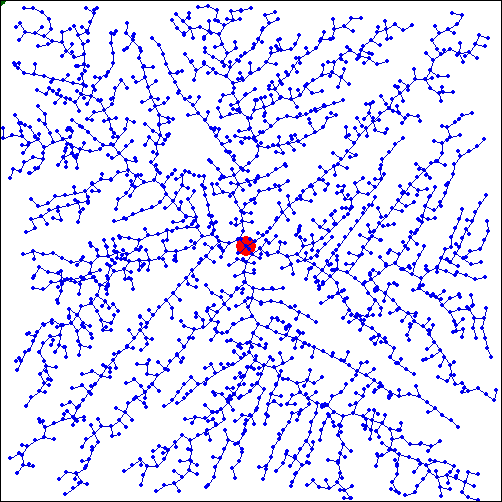
\includegraphics[width=\linewidth]{images/screenshot_41.png}
     \caption{2000 iterations}
  \end{subfigure}
  \hfill
  \begin{subfigure}[b]{0.3\linewidth}
    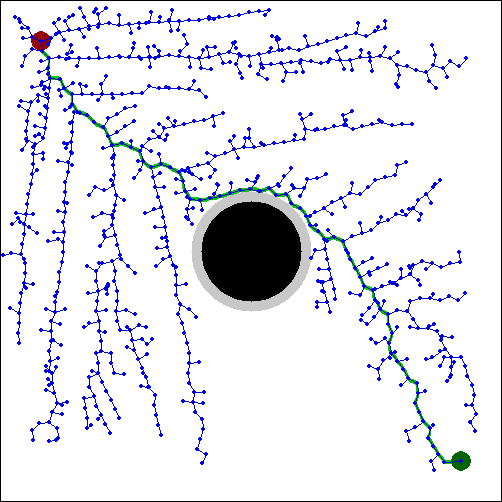
\includegraphics[width=\linewidth]{images/screenshot_39.png}
     \caption{Full RRT}
  \end{subfigure}
  \caption{RRT run with 500 iterations (left) and with 2000 iterations (middle) with $max\_dist$ 10. The whole algorithm can be seen in the right figure. Blue dots represent vertices and blue lines represent edges}
  \label{fig:RRT_example}
\end{figure}

\begin{algorithm}
\caption{Rapidly-exploring Random Tree (RRT)}
\label{alg: RRT}
\begin{algorithmic}[1]

\Procedure{RRT}{$M\colon(A, Os, G)$}
    \State $max\_dist \gets$ maximum distance
    allowed between tree children and sample
    \State $G \gets$ initalize graph with $A$ as vertex
    \While {True}
        \State $x_{rand} \gets \textit{Sample}()$
        \State $x_{near} \gets \textit{GetNearestVertex}(x_{rand})$
        \State $x_{new} \gets \textit{GetNewVertex}(x_{near}, x_{rand}, max\_dist)$
        \State
        \If {$\textit{CollisionFree}(x_{near}, x_{new})$}
            \State add $x_{new}$ as a new vertex to $G$
            \State add $(x_{near}, x_{new})$ as a new edge to $G$
        \EndIf
        \State
        \If {$x_{new}$ is in $G$ region}
            \State follow trace from root $G$ to $x_{new}$
            \State \Return 
        \EndIf
    \EndWhile
\EndProcedure
\end{algorithmic}
\end{algorithm}

Space complexity is $\mathcal{O}(|V| + |E|)$, where $|V|$ is the number of nodes and $|E|$ is the number of edges in graph $G$. Time complexity is given by $\mathcal{O}(i (\mathcal{O}(Sample) + \mathcal{O}(GetNearestVertex) + \mathcal{O}(GetNewVertex) + \mathcal{O}(CollisionFree)))$, where $i$ is the number of iterations and $\mathcal{O}(x)$ is the time complexity of method $x$. $i$ can be bounded by the number of nodes from graph $G$ ($\mathcal{O}(|V|)$) (at each step we add a new node to the graph). $\mathcal{O}(Sample)$ depends on the choice of sampling method (we use uniform random sampling which is $\mathcal{O}(1)$). $\mathcal{O}(GetNearestVertex)$ has DFS time and space complexity which is $\mathcal{O}(b^d)$ and $\mathcal{O}(bd)$, where $b$ is branching factor and $d$ is depth (if pruning is used $b$ becomes $\hat{b}$). $\mathcal{O}(GetNewVertex)$ is $\mathcal{O}(1)$ as it is a simple logical decision. $\mathcal{O}(CollisionFree)$ depends on the collision detection system. There are collision systems that have $\mathcal{O}(n)$ time complexity (for all entities). Because we need to check the path between $x_{near}$ and $x_{new}$ we still have $\mathcal{O}(n)$ time complexity. Therefore, the final time complexity is given by $\mathcal{O}(|V|(\mathcal{O}(b^d) + \mathcal{O}(n)))$.

A major advantage of using this method is that it is quite fast and memory efficient since it is run on a subset of the grid (the samples). Moreover, the algorithm can be coupled with the algorithms described in the Section \ref {C. Interpolating curve planners} (\hyperref[C. Interpolating curve planners]{Interpolating Curve Planners}) by transforming the graph edges into curves, which offers support for non-holonomic robots.

A major disadvantage is that, although the algorithm is probabilistic complete (as more samples are drawn the more likely is to find a path to the goal), it does not find an optimal path and the solution is usually quite jerky.

To overcome this issues, we introduce the RRT* \cite{karaman2011sampling, gammell2014informed} algorithm which has been proven to be asymptotic optimal (as the number of iterations gets larger, the more we approach to the optimal solution). RRT* does this by incrementally modifying the structure of the graph. When a new node is affixed to the graph, the algorithm might choose to rewire the connections in the graph by considering the new node as a replacement parent for the other existing nodes, if the resulting change yields a better solution. 

A major drawback of using RRT* is that, in order to achieve an optimal solution, the number of iterations has to be quite large and therefore, it becomes quickly expensive in higher dimensions. The Informed RRT* \cite{karaman2011sampling} algorithm attempts to solve this issue by adopting an ellipsoid heuristic approach. The algorithm shares the same logic as RRT* and it only improves the performance of finding an optimal path once a solution is found. This is achieved by sampling from the ellipsoidal heuristic. Thus, the number of iterations is reduced, and the optimal search is focused on a smaller region.

% \subsection{RRT*}

% Therefore, we introduce the RRT* \cite{karaman2011sampling} algorithm which is asymptotic optimal (as the problem size gets bigger, the more we approach to the optimal solution).

% % - prefers exploring the unexplored regions, large vornoi gaps
% % - good sampling from a smooth pdf Poisson Disc Sampling
% % - single nearest-neighbour queries

% \subsection{Informed RRT*}
% The informed RRT* \cite{gammell2014informed}
% %\subsection{Basic Probabilistic Road Map (Basic PRM)}
\section{Interpolating Curve Planners} \label{C. Interpolating curve planners}

% \todo{Add more citations}

The algorithms that lie into this section are used in the local planning part of the pathfinding problem. They attempt to find a trajectory that fits a given global description of the path (such as way-points) by taking into account multiple parameters such as feasibility, comfort, vehicle dynamics and efficiency. Interpolation is used to increase the number of data points between the way-points in order to smooth out the trajectory and create easily traversable paths for non-holonomic robots \cite{gonzalez2016review}.

\textbf{Lines and Circles.} Primitives such as lines and circles can be used to describe the local path between two way-points. Figure \ref{fig:c_all_curve_planners}(a) represents the shortest path to execute a 3-step 180\degree turn for a car. Because it can only fit geometric primitives, the algorithm is simple to implement and fast, but it is also quite limited (preferential parameters such as curvature angle and continuation are completely ignored).

\textbf{Clothoid Curves.} The implementation of this algorithm is based on Fresnel integrals, and the resulting curves offer a smoother transition between different curvatures (such as between a straight line and a curve) than Lines and Circles (See Figure \ref{fig:c_all_curve_planners}(b)). The algorithm accounts for multiple constraints such as dynamic and physical vehicle limitations (e.g. steering wheel), thus making it more robust for non-holonomic robots such as a car. Moreover, the algorithm was used in the design of highways and railways.

\textbf{Polynomial Curves.} This type of curves are mainly used to satisfy different preferential parameters such as angle and curvature when drawing the trajectory between two way-points. The main advantage of using this method is that the preferential parameters determine the coefficients of the polynomial, and thus, it is much more flexible. Figure \ref{fig:c_all_curve_planners}(c) represents an example of using polynomial curves to change lanes.

\textbf{Bézier Curves.} This algorithm produces curves based on control points. The control points placement defines the curvature at the beginning and the end of the curve.  The significant advantage of this algorithm is that it has a low computational cost since the shape of the curve is defined by the control points. Therefore, the algorithm has been extensively used in different drawing software applications, technical drawing (they can also be drawn by hand) and trajectory design. Moreover, the curve can be used to approximate clothoid curves. Figure \ref{fig:c_all_curve_planners}(d) represents an example of using 3rd and 4th degree Béziers to find the best curvature estimate based on the current situation.

\textbf{Spline Curves.} The spline curve is sub-divided into multiple parametric patches that can be defined as polynomial curves, clothoid curves and b-splines (Bézier curves). Splines have a high degree of smoothness at each patch joint and can be extended into higher dimensions. Figure \ref{fig:c_all_curve_planners}(e) represents an example of a b-spline with a changing knot (the junction between two sub-segments).

It is worth mentioning that the global description of the path demands to include the collision-free areas in addition to the way-points or provide a collision detection system to be used when drawing the curves to ensure that no collisions are encountered while performing any of the above algorithms.

\begin{figure}[h!]
  \centering
  \begin{subfigure}[b]{0.22\linewidth}
    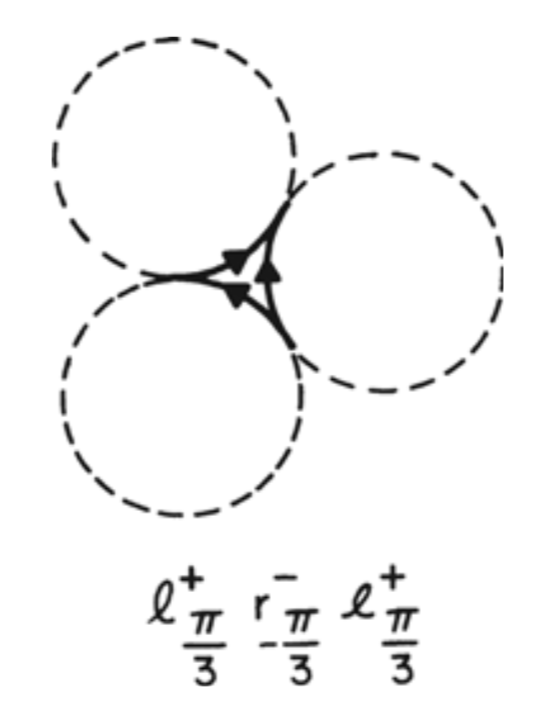
\includegraphics[width=\linewidth]{images/c_lines_and_circles.png}
     \caption{Lines and Circles \cite{gonzalez2016review}}
  \end{subfigure}
  \hfill
  \begin{subfigure}[b]{0.33\linewidth}
    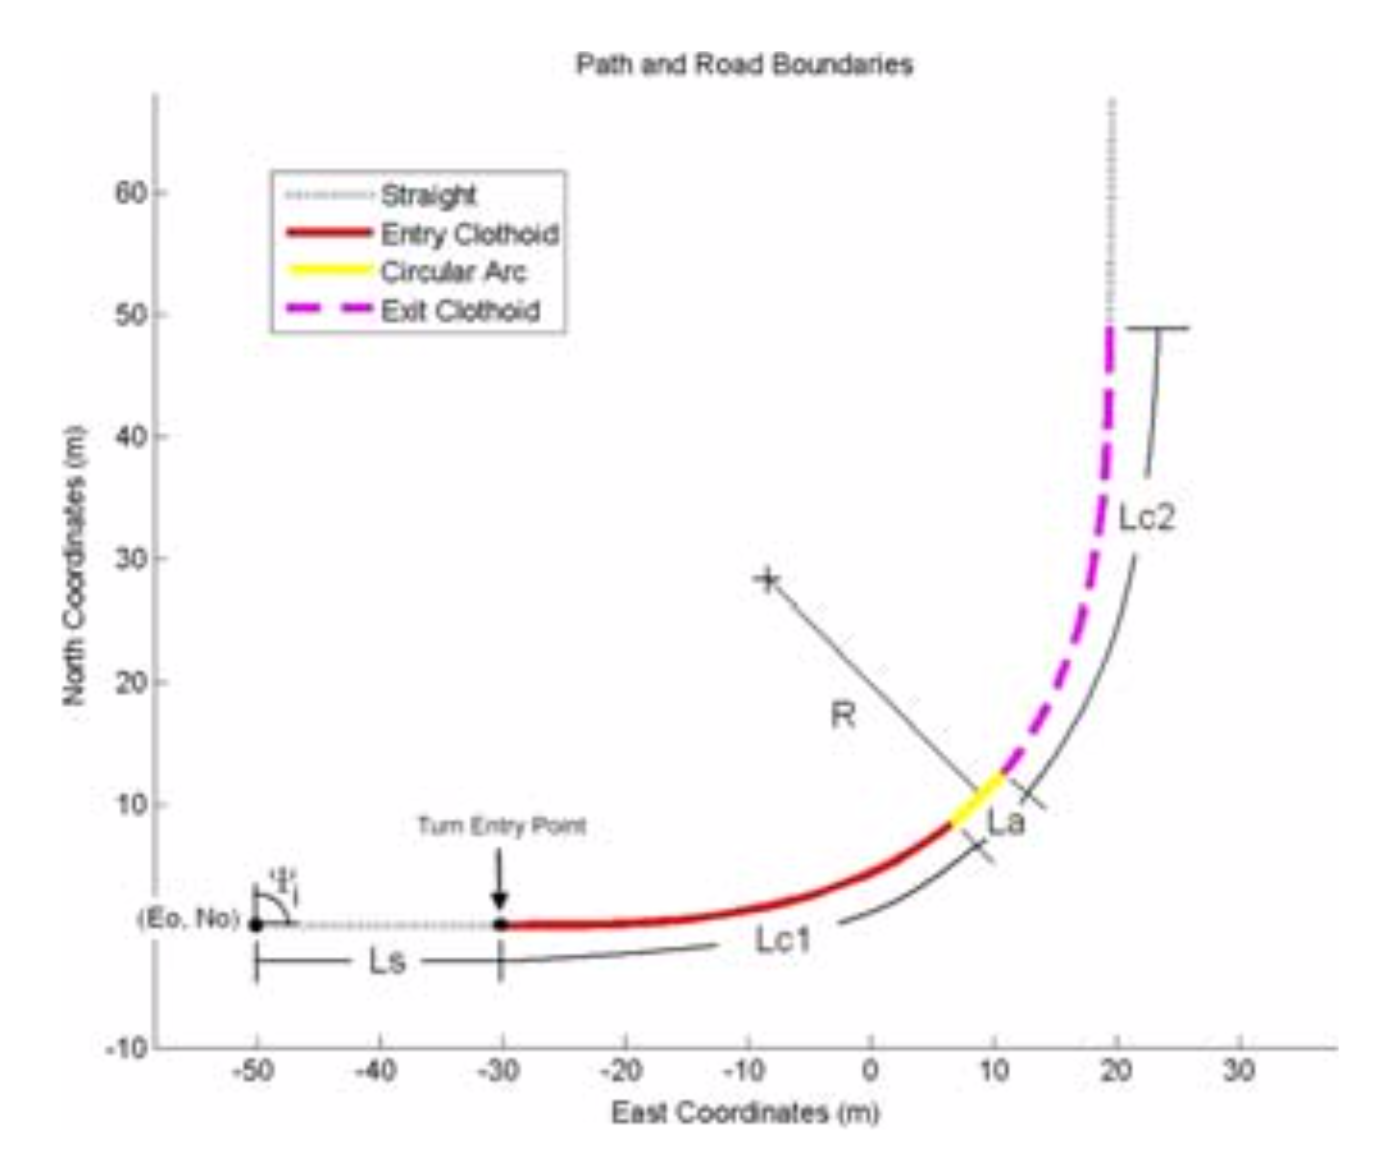
\includegraphics[width=\linewidth]{images/c_clothoid.png}
     \caption{Clothoid \cite{gonzalez2016review}}
  \end{subfigure}
  \hfill
  \begin{subfigure}[b]{0.38\linewidth}
    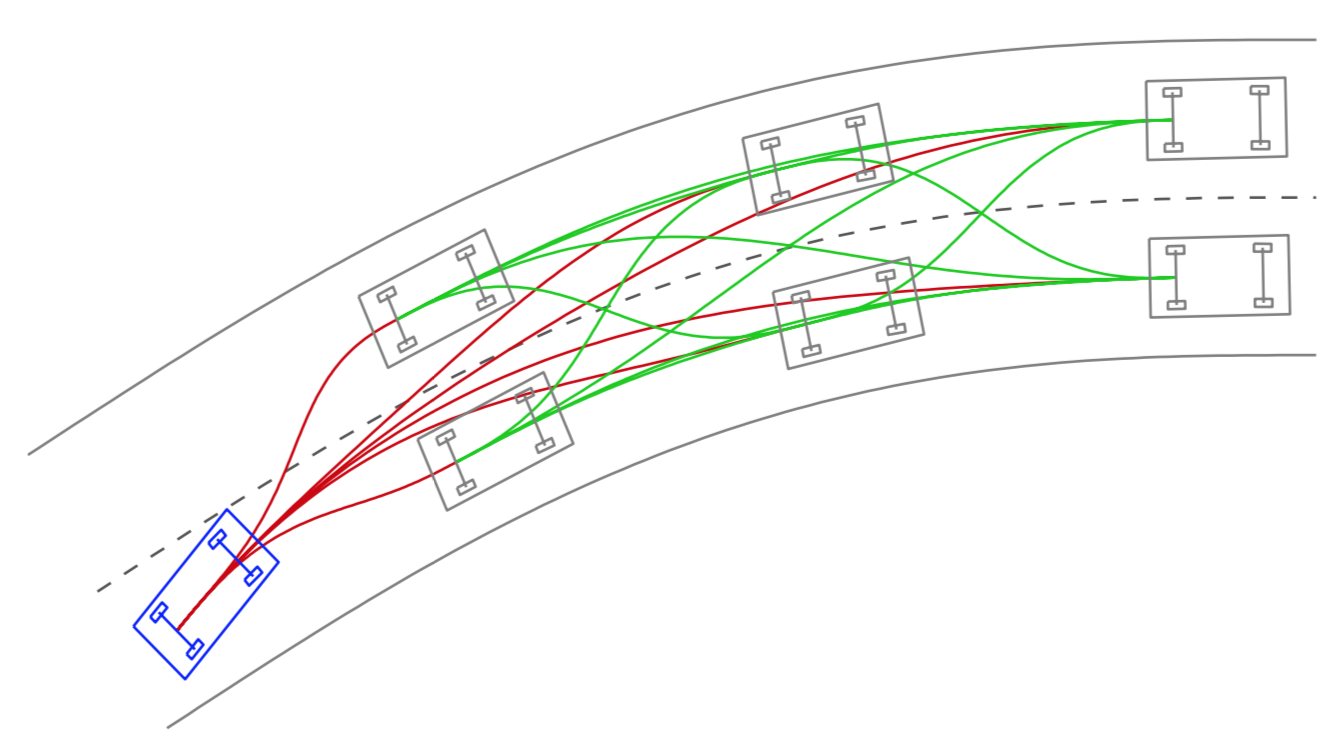
\includegraphics[width=\linewidth]{images/c_polynomial.png}
    \caption{Polynomial \cite{gonzalez2016review}}
  \end{subfigure}
  \newline
  \begin{subfigure}[b]{0.28\linewidth}
    \includegraphics[width=\linewidth]{images/c_bezier.png}
     \caption{Bézier \cite{gonzalez2016review}}
  \end{subfigure}
  \hspace{1cm}
  \begin{subfigure}[b]{0.33\linewidth}
    \includegraphics[width=\linewidth]{images/c_splines.png}
     \caption{Spline \cite{gonzalez2016review}}
  \end{subfigure}
  \caption{Examples of the most important interpolating curve planners}
  \label{fig:c_all_curve_planners}
\end{figure}
\section{Numerical Optimization Approaches} \label{D. Numerical optimization approaches}
This category of algorithms describes the path planning problem as a cost function, which is then minimised by using function approximation techniques and machine learning methods.

\subsection{Potential Field Method}
The main concept of the Potential Field Method (PFM) \cite{gonzalez2016review, ge2002dynamic, barraquand1992numerical} algorithm is to fill the map with a potential field $f$ in which the robot is attracted towards the goal and repulsed from obstacles. The potential field $f$ is composed of two functions: $f = a + r$ where $a$ is the attraction function and $r$ is the repulsion function. After the potential function is computed, an optimisation technique of finding the minimum of $f$, such as gradient descent, is applied (See Figure \ref{fig:pfm}). The Wave-front Planner \ref{sec: wave-front} is an example of a potential function $f=a$ where the repulsion function is missing.

The space complexity is $\mathcal{O}(nm)$ where $n$ is the width and $m$ is the height of the map. The time complexity is $\mathcal{O}(\mathcal{O}(f) + \mathcal{O}(gradient\_descent))$. $\mathcal{O}(f) = \mathcal{O}(\mathcal{O}(a) + \mathcal{O}(r))$ depends on the choice of $a$ and $r$. Assuming same $a$ as in the Wave-front Planner, $\mathcal{O}(a) = \mathcal{O}(b^d)$, where $b$ is the branching factor and $d$ is the depth. Assuming that we use a simple $r$ which inflates the obstacle, the time complexity of $\mathcal{O}(r)$ is $\mathcal{O}(xo)$, where $x$ is the inflation rate and $o$ is the average obstacle size. $\mathcal{O}(gradient\_descent)$ is more involved if we use real gradient descent optimisation as it is based on the convergence rate. If we were to use the same gradient descent method from the Wave-front Planner, then $\mathcal{O}(gradient\_descent) = \mathcal{O}(d)$, where $d$ is the depth of the solution. The final time complexity is $\mathcal{O}(b^d + xo + d)$.

This solution is appealing because it is mathematically elegant and simple. It behaves well on complex environments which contain narrow passages, and it keeps a safe distance from the obstacles based on different factors such as relative velocity. Moreover, the algorithm can be extended to highly dynamic environments in which the obstacles and the goal are continually moving. Lastly, we can use vehicle parameters such as velocity and torque, to define $a$ and $r$. Thus, we can avoid collisions based on the velocity of the vehicle (i.e. when the vehicle has a high enough velocity to not being able to exit a collision trajectory) \cite{ge2002dynamic}.

One of the major drawbacks of using this method is that depending on the choice of $f$, local minimum problems might arise. Usually, these problems require particular solutions and rigorous analysis to ensure that there is no situation in which the agent will be trapped forever.

\begin{figure}[h!]
    \centering
    \includegraphics[scale=0.3]{images/pfm.png}
    \caption{Potential field $f = a + r$, where $a$ is the attraction function and $r$ is the repulsion function \cite{inproceedings}}
    \label{fig:pfm}
\end{figure}

\pagebreak

\subsection{LSTM}
Currently, the most important works that have considered LSTMs in this field are \cite{nicola2018lstm, lee2018lstm, inoue2019robot}.

%\cite{nicola2018lstm} uses an LSTM network to generate a path from the agent to the goal. The network was trained using A* on randomly generated maps and tested on maps from the online game Dragon Age. The issue with this approach is that the agent might get lost and will not succeed in finding a path to the goal, if there exists one. It has also been noticed that the algorithm has a higher success rate if the size of the map is relatively small and simple in layout.

Nicola et al. attempt to use an LSTM network to create an online global path planner by generating a low-resolution high-level path from start to goal \cite{nicola2018lstm}. The network was trained on randomly filled generated mazes with different corridor sizes with A* \ref{sec:a_star} as ground truth and tested on maps from the popular game Dragon Age. The primary motivation of using the proposed method from \cite{nicola2018lstm} is that, unlike A* which is offline (directly produces the final output), this method is an online search strategy that takes into account the fact that the environment is usually unknown or too expensive to store. Thus, at each time step, the network is queried for the next action that it should take given the local information of the map and previous choice of action. One of the significant drawbacks is that the rate of success of the algorithm gets lower as the map becomes more complicated (longer corridors, more complex objects).

Lee et al. make use of the LSTM architecture to extend the state of the art Value Iteration Networks (VIN) \cite{lee2018lstm}. VINs are similar to the Value Iteration algorithm described in \label{sec:vin} applied on a 2D grid world, but without making use of pre-defined MDP parameters such as the transition probabilities and rewards. The paper has pointed out that, despite being so successful, there are still issues with the current design of VIN such as the design of the transition model and the large number of recursive calls taken to achieve a reasonable estimate of the optimal path to the goal. The proposed solution replaces the recurrent VIN update rule with an LSTM kernel. \cite{lee2018lstm} has shown that the performance of the new solution has better or at least as good performance as the original VIN.

Inoue et al. aim to use a Convolutional Auto-encoder (CAE) combined with an LSTM to plan a path under a changing environment, by disregarding the unknown environment constraint (the map is fully discovered) \cite{inoue2019robot}. The two network sections are trained individually. Firstly, the CAE is trained on randomly generated maps with obstacles of different sizes. After that, the decoder is discarded, and the encoder is used to encode the same maps in order to extract the main features. Secondly, the LSTM is trained on the encoded maps by using RRT as ground truth. Unlike \cite{nicola2018lstm}, the solution is offline as it produces a full path (which might collide with obstacles), but it can be easily converted to an online solution in order to handle collision detection and prevention. A significant difference between this solution and \cite{nicola2018lstm} is that it has a higher overall success rate, which might arise since the CAE learns the input features as opposed to being hand crafted as in \cite{nicola2018lstm}.

%\cite{inoue2019robot} has a similar approach to \cite{nicola2018lstm}, but, in addition, it compares the LSTM network to a Value Iteration Network. The results show that the LSTM is, overall, better than the Value Iteration Network, but, still, they share the same issues as \cite{nicola2018lstm} (i.e. the algorithm has a low success rate of finding a path to the goal and if it finds one it is usually not optimal).


%\subsection{Machine Learning and Neural Networks methods}
%VIN (Value Iteration Networks)
%LSTMIN (Long Short Term Memory Iteration Networks)